\documentclass[11pt,a4paper]{article}
\usepackage[margin=1in]{geometry}
\usepackage{booktabs}
\usepackage{array}
\usepackage{longtable}
\usepackage{xcolor}
\usepackage{enumitem}
\usepackage{hyperref}
\usepackage{graphicx}
\usepackage{float}

\title{TaxiTap System\\Service Contracts Documentation}
\author{Software Requirements Specification}
\date{}

\begin{document}


\maketitle

\begin{figure}[H]
  \centering
  
\includegraphics[width=0.5\textwidth]{LogoGroup.png} 
\end{figure}

\begin{figure}[H]
  \centering
  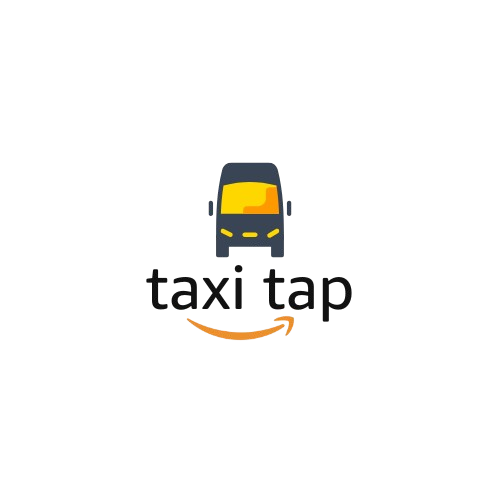
\includegraphics[width=0.5\textwidth]{LogoTaxiTap.png} 
\end{figure}

\newpage

\tableofcontents
\newpage

\section{Introduction}

This document provides service contracts for all major services within the TaxiTap ride-sharing system. Each service contract defines a clear and consistent description of how the service can be used, including its purpose, required inputs, expected outputs, and interactions with other system components.

Service contracts serve as API specifications that outline the interface and behavior expectations for each service, ensuring clear communication between different parts of the system and external integrators.

\section{User Account Management Service}

The User Account Management service handles all user-related operations including registration, authentication, profile management, and role switching functionality.

\subsection{signUpSMS Function}

\begin{longtable}{|p{4cm}|p{12cm}|}
\hline
\textbf{Field} & \textbf{Description} \\
\hline
\textbf{What the service does} & 
Registers a new user account in the TaxiTap system using SMS-based verification. Creates user profile with provided information and sends SMS verification code to the provided phone number. \\
\hline
\textbf{Inputs required} & 
\begin{itemize}[nosep]
\item \texttt{phoneNumber} (string) - Valid phone number in international format
\item \texttt{name} (string) - User's full name (2-0 characters)
\item \texttt{password} (string) - Secure password (minimum 8 characters)
\item \texttt{accountType} ("passenger" | "driver" | "both") - Account role type
\item \texttt{email} (optional string) - Valid email address
\item \texttt{age} (optional number) - User age (must be 18 or older)
\end{itemize} \\
\hline
\textbf{Outputs returned} & 
\begin{itemize}[nosep]
\item \texttt{userId} (Id<"taxiTap\_users">) - Unique user identifier
\item \texttt{verificationStatus} (boolean) - SMS verification status
\item \texttt{sessionToken} (string) - Authentication token for session
\item \texttt{userProfile} (object) - Created user profile data
\item \texttt{success} (boolean) - Operation success indicator
\item \texttt{errorMessage} (optional string) - Error details if operation fails
\end{itemize} \\
\hline
\textbf{Interactions with other systems/components   } & 
\begin{itemize}[nosep]
\item Database Service - Stores user account data
\item Authentication Service - Authenticates user information
\item Validation Service - Validates input parameters
\item Notification System - Sends welcome notification
\end{itemize} \\
\hline
\end{longtable}

\subsection{loginSMS Function}

\begin{longtable}{|p{4cm}|p{12cm}|}
\hline
\textbf{Field} & \textbf{Description} \\
\hline
\textbf{What the service does} & 
Authenticates existing users using phone number and password combination. Validates credentials and establishes authenticated session with appropriate permissions based on user's account type. \\
\hline
\textbf{Inputs required} & 
\begin{itemize}[nosep]
\item \texttt{phoneNumber} (string) - Registered phone number
\item \texttt{password} (string) - User password
\end{itemize} \\
\hline
\textbf{Outputs returned} & 
\begin{itemize}[nosep]
\item \texttt{userId} (Id<"taxiTap\_users">) - Authenticated user identifier
\item \texttt{sessionToken} (string) - Authentication token for session
\item \texttt{userProfile} (object) - User profile information
\item \texttt{activeRole} ("passenger" | "driver") - Current active role
\item \texttt{permissions} (array) - User permission set
\item \texttt{success} (boolean) - Authentication result
\item \texttt{errorMessage} (optional string) - Error details if authentication fails
\end{itemize} \\
\hline
\textbf{Interactions with other systems/components} & 
\begin{itemize}[nosep]
\item Database Service - Retrieves and validates user credentials
\item Authentication Service - Generates and manages session tokens
\item Security Service - Logs authentication attempts
\item User Profile Service - Retrieves user profile data
\end{itemize} \\
\hline
\end{longtable}

\subsection{switchActiveRole Function}

\begin{longtable}{|p{4cm}|p{12cm}|}
\hline
\textbf{Field} & \textbf{Description} \\
\hline
\textbf{What the service does} & 
Allows users with multiple account types to switch between passenger and driver roles. Updates active permissions and interface preferences based on selected role. \\
\hline
\textbf{Inputs required} & 
\begin{itemize}[nosep]
\item \texttt{userId} (Id<"taxiTap\_users">) - Authenticated user identifier
\item \texttt{newRole} ("passenger" | "driver") - Target role to switch to
\end{itemize} \\
\hline
\textbf{Outputs returned} & 
\begin{itemize}[nosep]
\item \texttt{activeRole} ("passenger" | "driver") - Updated active role
\item \texttt{permissions} (array) - Updated permission set
\item \texttt{interfaceConfig} (object) - Role-specific UI configuration
\item \texttt{success} (boolean) - Role switch result
\item \texttt{errorMessage} (optional string) - Error details if switch fails
\end{itemize} \\
\hline
\textbf{Interactions with other systems/components} & 
\begin{itemize}[nosep]
\item Authentication Service - Updates session permissions
\item Database Service - Updates user's active role status
\item UI Configuration Service - Provides role-specific interface settings
\item Activity Tracking Service - Logs role switch event
\end{itemize} \\
\hline
\end{longtable}

\subsection{updateUserProfile Function}

\begin{longtable}{|p{4cm}|p{12cm}|}
\hline
\textbf{Field} & \textbf{Description} \\
\hline
\textbf{What the service does} & 
Updates user profile information including personal details, contact information, and emergency contacts. Validates all changes and maintains data integrity across the system. \\
\hline
\textbf{Inputs required} & 
\begin{itemize}[nosep]
\item \texttt{userId} (Id<"taxiTap\_users">) - User identifier for profile update
\item \texttt{name} (string) - Updated full name
\item \texttt{phoneNumber} (string) - Updated phone number
\item \texttt{email} (optional string) - Updated email address
\item \texttt{profilePicture} (optional string) - Profile image URL or base64 data
\item \texttt{emergencyContact} (optional object) - Emergency contact details:
  \begin{itemize}[nosep]
    \item \texttt{name} (string) - Contact person's name
    \item \texttt{phoneNumber} (string) - Contact phone number
    \item \texttt{relationship} (string) - Relationship to user
  \end{itemize}
\end{itemize} \\
\hline
\textbf{Outputs returned} & 
\begin{itemize}[nosep]
\item \texttt{updatedProfile} (object) - Complete updated user profile
\item \texttt{changedFields} (array) - List of fields that were modified
\item \texttt{validationErrors} (array) - Any validation issues encountered
\item \texttt{success} (boolean) - Update operation result
\item \texttt{errorMessage} (optional string) - Error details if update fails
\end{itemize} \\
\hline
\textbf{Interactions with other systems/components} & 
\begin{itemize}[nosep]
\item Database Service - Persists profile changes
\item Validation Service - Validates all input data
\item Image Processing Service - Processes profile picture uploads
\item Notification System - Notifies user of successful profile updates
\item Security Service - Logs profile modification events
\end{itemize} \\
\hline
\end{longtable}

\section{Ride Request System Service}

The Ride Request System service manages the complete ride request lifecycle from initial passenger request through driver matching, ride execution, and completion. This service consists of multiple handler functions that coordinate real-time interactions between passengers and drivers.

\subsection{requestRideHandler Function}

\begin{longtable}{|p{4cm}|p{12cm}|}
\hline
\textbf{Field} & \textbf{Description} \\
\hline
\textbf{What the service does} & 
Initiates a new ride request from a passenger. Creates a ride record, calculates fare estimates, searches for available drivers in the vicinity, and broadcasts the ride request to eligible drivers. Manages the initial matching process and sets up real-time tracking. \\
\hline
\textbf{Inputs required} & 
\begin{itemize}[nosep]
\item \texttt{passengerId} (string) - Unique identifier of the requesting passenger
\item \texttt{driverId} (string) - Specific driver identifier if passenger has a preference
\item \texttt{startLocation} (object) - Pickup location details:
  \begin{itemize}[nosep]
    \item \texttt{coordinates} (object) - Latitude and longitude coordinates
    \item \texttt{address} (string) - Human-readable pickup address
  \end{itemize}
\item \texttt{endLocation} (object) - Destination location details:
  \begin{itemize}[nosep]
    \item \texttt{coordinates} (object) - Latitude and longitude coordinates
    \item \texttt{address} (string) - Human-readable destination address
  \end{itemize}
\item \texttt{estimatedFare} (optional number) - Pre-calculated fare estimate
\item \texttt{estimatedDistance} (optional number) - Pre-calculated distance in kilometers
\item \texttt{estimatedDuration} (optional number) - Pre-calculated duration in minutes
\end{itemize} \\
\hline
\textbf{Outputs returned} & 
\begin{itemize}[nosep]
\item \texttt{rideId} (string) - Unique identifier for the created ride request
\item \texttt{requestStatus} ("created" | "searching" | "pending\_driver\_response") - Current request status
\item \texttt{estimatedMatchTime} (number) - Expected time to find a driver in minutes
\item \texttt{nearbyDrivers} (array) - List of available drivers in the area
\item \texttt{fareDetails} (object) - Detailed fare breakdown including base fare, taxes, and fees
\item \texttt{routePreview} (object) - Basic route information and map data
\item \texttt{success} (boolean) - Request creation result
\item \texttt{errorMessage} (optional string) - Error details if request fails
\end{itemize} \\
\hline
\textbf{Interactions with other systems/components} & 
\begin{itemize}[nosep]
\item Database Service - Creates ride record and retrieves passenger details
\item Driver Matching Service - Finds and filters available drivers
\item Routes Service - Calculates route and fare estimates
\item Notification System - Sends ride requests to drivers
\item Real-time Tracking Service - Initializes location tracking
\item Geolocation Service - Validates and processes location data
\item Fare Calculation Service - Computes accurate pricing
\end{itemize} \\
\hline
\end{longtable}

\subsection{acceptRideHandler Function}

\begin{longtable}{|p{4cm}|p{12cm}|}
\hline
\textbf{Field} & \textbf{Description} \\
\hline
\textbf{What the service does} & 
Processes a driver's acceptance of a ride request. Updates ride status, establishes the passenger-driver connection, cancels notifications to other drivers, and initiates the active ride phase with real-time coordination. \\
\hline
\textbf{Inputs required} & 
\begin{itemize}[nosep]
\item \texttt{rideId} (string) - Unique identifier of the ride request being accepted
\item \texttt{driverId} (string) - Unique identifier of the driver accepting the ride
\end{itemize} \\
\hline
\textbf{Outputs returned} & 
\begin{itemize}[nosep]
\item \texttt{rideStatus} ("accepted" | "driver\_en\_route") - Updated ride status
\item \texttt{driverDetails} (object) - Complete driver profile and vehicle information
\item \texttt{estimatedArrival} (datetime) - Expected driver arrival time at pickup location
\item \texttt{trackingInfo} (object) - Real-time tracking details for passenger
\item \texttt{contactInfo} (object) - Secure communication channels between passenger and driver
\item \texttt{ridePin} (string) - Security PIN for ride verification
\item \texttt{success} (boolean) - Acceptance processing result
\item \texttt{errorMessage} (optional string) - Error details if acceptance fails
\end{itemize} \\
\hline
\textbf{Interactions with other systems/components} & 
\begin{itemize}[nosep]
\item Database Service - Updates ride status and driver assignment
\item Notification System - Notifies passenger of driver acceptance and cancels other driver notifications
\item Real-time Tracking Service - Activates live location sharing
\item Driver Availability Service - Updates driver status to busy
\item Communication Service - Establishes secure passenger-driver communication
\item Route Optimization Service - Provides optimal route to pickup location
\end{itemize} \\
\hline
\end{longtable}

\subsection{cancelRideHandler Function}

\begin{longtable}{|p{4cm}|p{12cm}|}
\hline
\textbf{Field} & \textbf{Description} \\
\hline
\textbf{What the service does} & 
Handles ride cancellation requests from either passengers or drivers. Processes cancellation fees if applicable, updates all parties involved, releases driver availability, and manages refunds or charges based on cancellation policy and timing. \\
\hline
\textbf{Inputs required} & 
\begin{itemize}[nosep]
\item \texttt{rideId} (string) - Unique identifier of the ride to be cancelled
\item \texttt{userId} (string) - Identifier of the user initiating the cancellation (passenger or driver)
\end{itemize} \\
\hline
\textbf{Outputs returned} & 
\begin{itemize}[nosep]
\item \texttt{cancellationStatus} ("cancelled" | "cancellation\_failed") - Result of cancellation attempt
\item \texttt{affectedParties} (array) - List of users notified about the cancellation
\item \texttt{driverCompensation} (optional object) - Compensation for driver if applicable
\item \texttt{success} (boolean) - Cancellation processing result
\item \texttt{errorMessage} (optional string) - Error details if cancellation fails
\end{itemize} \\
\hline
\textbf{Interactions with other systems/components} & 
\begin{itemize}[nosep]
\item Database Service - Updates ride status and records cancellation details
\item Payment System - Processes cancellation fees and refunds
\item Notification System - Notifies all affected parties of cancellation
\item Seat Availability Service - Updates driver seat status back to available
\item Real-time Tracking Service - Terminates active tracking sessions
\end{itemize} \\
\hline
\end{longtable}

\subsection{completeRideHandler Function}

\begin{longtable}{|p{4cm}|p{12cm}|}
\hline
\textbf{Field} & \textbf{Description} \\
\hline
\textbf{What the service does} & 
Finalizes a ride when the driver marks it as completed after reaching the destination. Calculates final fare based on actual route and time, processes payment, updates driver availability, and triggers post-ride activities like rating requests. \\
\hline
\textbf{Inputs required} & 
\begin{itemize}[nosep]
\item \texttt{rideId} (string) - Unique identifier of the ride being completed
\item \texttt{driverId} (string) - Identifier of the driver marking the ride as complete
\end{itemize} \\
\hline
\textbf{Outputs returned} & 
\begin{itemize}[nosep]
\item \texttt{rideStatus} ("completed") - Final ride status
\item \texttt{finalFare} (object) - Complete fare breakdown including actual charges
\item \texttt{paymentStatus} ("processed" | "pending" | "failed") - Payment processing result
\item \texttt{rideHistory} (object) - Complete ride details for records
\item \texttt{receiptInfo} (object) - Digital receipt details
\item \texttt{driverEarnings} (object) - Driver earnings breakdown
\item \texttt{ratingPrompt} (boolean) - Whether rating requests should be sent
\item \texttt{success} (boolean) - Completion processing result
\end{itemize} \\
\hline
\textbf{Interactions with other systems/components} & 
\begin{itemize}[nosep]
\item Database Service - Updates ride completion status and stores final details
\item Payment System - Processes final payment and driver earnings
\item Notification System - Sends completion notifications and rating requests
\item Real-time Tracking Service - Finalizes tracking data
\end{itemize} \\
\hline
\end{longtable}

\subsection{declineRideHandler Function}

\begin{longtable}{|p{4cm}|p{12cm}|}
\hline
\textbf{Field} & \textbf{Description} \\
\hline
\textbf{What the service does} & 
Processes a driver's decision to decline a ride request. Records the decline reason, removes the driver from the current request pool, continues searching for alternative drivers, and may adjust driver matching algorithms based on decline patterns. \\
\hline
\textbf{Inputs required} & 
\begin{itemize}[nosep]
\item \texttt{rideId} (string) - Unique identifier of the ride request being declined
\item \texttt{driverId} (string) - Identifier of the driver declining the ride
\end{itemize} \\
\hline
\textbf{Outputs returned} & 
\begin{itemize}[nosep]
\item \texttt{declineStatus} ("declined") - Confirmation of decline processing
\item \texttt{remainingDrivers} (array) - List of other drivers still available for the ride
\item \texttt{searchContinues} (boolean) - Whether the search for drivers continues
\item \texttt{estimatedMatchTime} (number) - Updated estimated time to find a driver
\item \texttt{driverAvailability} ("available" | "temporarily\_unavailable") - Driver's updated availability status
\item \texttt{success} (boolean) - Decline processing result
\item \texttt{errorMessage} (optional string) - Error details if decline processing fails
\end{itemize} \\
\hline
\textbf{Interactions with other systems/components} & 
\begin{itemize}[nosep]
\item Database Service - Records decline and updates ride request status
\item Driver Matching Service - Continues search with remaining drivers
\item Analytics Service - Records decline patterns for algorithm improvement
\item Notification System - May notify passenger of continued search
\end{itemize} \\
\hline
\end{longtable}

\subsection{endRideHandler Function}

\begin{longtable}{|p{4cm}|p{12cm}|}
\hline
\textbf{Field} & \textbf{Description} \\
\hline
\textbf{What the service does} & 
Handles the final termination of a ride session, typically called after completion processing. Cleans up active sessions, terminates real-time connections, archives ride data, and ensures all resources are properly released for system efficiency. \\
\hline
\textbf{Inputs required} & 
\begin{itemize}[nosep]
\item \texttt{rideId} (string) - Unique identifier of the ride session to end
\item \texttt{userId} (string) - Identifier of the user requesting to end the ride session
\end{itemize} \\
\hline
\textbf{Outputs returned} & 
\begin{itemize}[nosep]
\item \texttt{sessionStatus} ("ended") - Confirmation that ride session has been terminated
\item \texttt{dataArchived} (boolean) - Whether ride data has been successfully archived
\item \texttt{resourcesReleased} (boolean) - Confirmation of system resource cleanup
\item \texttt{finalSummary} (object) - Complete ride summary for user records
\item \texttt{nextActions} (array) - Available post-ride actions (rate, report, share)
\item \texttt{success} (boolean) - Session termination result
\item \texttt{errorMessage} (optional string) - Error details if termination fails
\end{itemize} \\
\hline
\textbf{Interactions with other systems/components} & 
\begin{itemize}[nosep]
\item Database Service - Archives ride data and cleans active sessions
\item Real-time Tracking Service - Terminates location tracking and connections
\item Session Management Service - Ends active ride sessions
\item Resource Management Service - Releases allocated system resources
\item Cache Service - Clears temporary ride-related cached data
\item Monitoring Service - Updates system performance metrics
\item Cleanup Service - Performs post-ride system maintenance tasks
\end{itemize} \\
\hline
\end{longtable}

\section{Notification System Service}

The Notification System service manages all communication between the system and users through multiple channels including SMS, push notifications, and in-app messages. This service handles notification delivery, user preferences, and message tracking.

\subsection{sendNotificationHandler Function}

\begin{longtable}{|p{4cm}|p{12cm}|}
\hline
\textbf{Field} & \textbf{Description} \\
\hline
\textbf{What the service does} & 
Sends notifications to users through appropriate channels based on user preferences and message type. Handles message formatting, delivery method selection, queuing for reliable delivery, and tracks delivery status across multiple notification channels. \\
\hline
\textbf{Inputs required} & 
\begin{itemize}[nosep]
\item \texttt{userId} (string) - Unique identifier of the target user
\item \texttt{message} (string) - The notification message content to be sent
\item \texttt{type} (string) - Notification category such as "ride", "payment", "system"
\item \texttt{metadata} (optional object) - Additional data for message customization and tracking
\end{itemize} \\
\hline
\textbf{Outputs returned} & 
\begin{itemize}[nosep]
\item \texttt{notificationId} (string) - Unique identifier for the sent notification
\item \texttt{deliveryStatus} ("queued" | "sent" | "delivered" | "failed") - Current delivery status
\item \texttt{deliveryMethod} (string) - Method used for delivery (SMS, push, in-app, email)
\item \texttt{deliveryTimestamp} (datetime) - When the notification was sent
\item \texttt{estimatedDelivery} (datetime) - Expected delivery time
\item \texttt{retryCount} (number) - Number of delivery attempts if failed
\item \texttt{success} (boolean) - Notification sending result
\item \texttt{errorMessage} (optional string) - Error details if sending fails
\end{itemize} \\
\hline
\textbf{Interactions with other systems/components} & 
\begin{itemize}[nosep]
\item Database Service - Stores notification records and retrieves user preferences
\item SMS Gateway - Sends SMS notifications
\item Push Notification Service - Delivers mobile push notifications
\item Email Service - Sends email notifications
\item User Preferences Service - Determines preferred notification channels
\item Template Engine - Formats messages using predefined templates
\item Queue Management Service - Manages notification delivery queues
\item Analytics Service - Tracks notification metrics and engagement
\end{itemize} \\
\hline
\end{longtable}

\subsection{getNotificationsHandler Function}

\begin{longtable}{|p{4cm}|p{12cm}|}
\hline
\textbf{Field} & \textbf{Description} \\
\hline
\textbf{What the service does} & 
Retrieves a user's notification history including unread messages, notification status, and metadata. Supports pagination for large notification lists and provides filtering options by notification type, date range, and read status. \\
\hline
\textbf{Inputs required} & 
\begin{itemize}[nosep]
\item \texttt{userId} (string) - Unique identifier of the user whose notifications to retrieve
\end{itemize} \\
\hline
\textbf{Outputs returned} & 
\begin{itemize}[nosep]
\item \texttt{notifications} (array) - List of user notifications with details
\item \texttt{unreadCount} (number) - Total number of unread notifications
\item \texttt{totalCount} (number) - Total number of notifications for the user
\item \texttt{latestNotification} (object) - Most recent notification details
\item \texttt{notificationTypes} (array) - Available notification categories
\item \texttt{paginationInfo} (object) - Pagination details for large lists
\item \texttt{success} (boolean) - Retrieval operation result
\item \texttt{errorMessage} (optional string) - Error details if retrieval fails
\end{itemize} \\
\hline
\textbf{Interactions with other systems/components} & 
\begin{itemize}[nosep]
\item Database Service - Retrieves stored notification records
\item User Authentication Service - Validates user identity and permissions
\item Pagination Service - Handles large result set pagination
\item Notification Filtering Service - Applies filters and sorting options
\item Cache Service - Caches frequently accessed notification data
\item Analytics Service - Tracks notification access patterns
\end{itemize} \\
\hline
\end{longtable}

\subsection{markNotificationAsReadHandler Function}

\begin{longtable}{|p{4cm}|p{12cm}|}
\hline
\textbf{Field} & \textbf{Description} \\
\hline
\textbf{What the service does} & 
Updates the read status of a specific notification when a user views it. Records the read timestamp, updates unread counts, and may trigger follow-up actions based on notification type. Ensures accurate tracking of user engagement with notifications. \\
\hline
\textbf{Inputs required} & 
\begin{itemize}[nosep]
\item \texttt{notificationId} (string) - Unique identifier of the notification to mark as read
\item \texttt{userId} (string) - Identifier of the user marking the notification as read
\end{itemize} \\
\hline
\textbf{Outputs returned} & 
\begin{itemize}[nosep]
\item \texttt{readStatus} ("read") - Confirmation that notification has been marked as read
\item \texttt{readTimestamp} (datetime) - When the notification was marked as read
\item \texttt{updatedUnreadCount} (number) - New unread notification count for the user
\item \texttt{followUpActions} (array) - Any triggered actions based on the notification type
\item \texttt{notificationDetails} (object) - Updated notification information
\item \texttt{success} (boolean) - Read status update result
\item \texttt{errorMessage} (optional string) - Error details if update fails
\end{itemize} \\
\hline
\textbf{Interactions with other systems/components} & 
\begin{itemize}[nosep]
\item Database Service - Updates notification read status and timestamp
\item User Authentication Service - Validates user permissions for the notification
\item Analytics Service - Tracks notification engagement and read patterns
\item Counter Service - Updates unread notification counters
\item Follow-up Action Service - Triggers actions based on notification type
\item Cache Service - Updates cached notification status data
\end{itemize} \\
\hline
\end{longtable}

\section{Routes Service}


\subsection{calculateRoute Function}

\begin{longtable}{|p{4cm}|p{12cm}|}
\hline
\textbf{Field} & \textbf{Description} \\
\hline
\textbf{Service Name} & findBestMatchingRoutes \\
\hline
\textbf{What the service does} & 
Finds optimal transportation routes based on geographical proximity to user-specified start and end locations. Calculates distance-based scores using Haversine formula, filters routes within configurable distance limits, and returns routes sorted by suitability with comprehensive proximity metrics and stop details. \\
\hline
\textbf{Inputs required} & 
\begin{itemize}[nosep]
\item \texttt{startLat} (number) - Latitude of departure location
\item \texttt{startLon} (number) - Longitude of departure location
\item \texttt{endLat} (number) - Latitude of destination location
\item \texttt{endLon} (number) - Longitude of destination location
\item \texttt{maxStartDistance} (optional number) - Maximum acceptable distance from start point in km (default: 2.0)
\item \texttt{maxEndDistance} (optional number) - Maximum acceptable distance from end point in km (default: 8.0)
\item \texttt{maxResults} (optional number) - Maximum routes to return (default: 10)
\end{itemize} \\
\hline
\textbf{Outputs returned} & 
\begin{itemize}[nosep]
\item \texttt{success} (boolean) - Operation status
\item \texttt{matchingRoutes} (array) - Optimized route recommendations with:
  \begin{itemize}[nosep]
  \item Route identification and metadata
  \item Proximity measurements to start/end points
  \item Closest stop details with distances
  \item Route suitability scoring
  \item Direct route availability flag
  \end{itemize}
\item \texttt{totalRoutesChecked} (number) - Total active routes evaluated
\item \texttt{routesWithinRange} (number) - Routes meeting distance criteria
\item \texttt{searchCriteria} (object) - Parameters used for search
\item \texttt{message} (string) - Status or error information
\end{itemize} \\
\hline
\textbf{Interactions with other systems/components} & 
\begin{itemize}[nosep]
\item Route Database - Retrieves all active routes
\item Enriched Stops Database - Gets enhanced stop information
\item Distance Calculation Service - Haversine formula computations
\item Scoring Engine - Calculates route suitability scores
\item Filtering Service - Applies distance constraints
\item Sorting Service - Orders results by priority
\end{itemize} \\
\hline
\end{longtable}

\subsection{displayRoute Function}

\begin{longtable}{|p{4cm}|p{12cm}|}
\hline
\textbf{Field} & \textbf{Description} \\
\hline
\textbf{What the service does} & 
Provides comprehensive details for a specific route including all stops with optional distance calculations from a user's current location. Retrieves enriched stop information and calculates proximity metrics when user coordinates are provided. \\
\hline
\textbf{Inputs required} & 
\begin{itemize}[nosep]
\item \texttt{routeId} (string) - Unique identifier of the target route
\item \texttt{userLat} (optional number) - User's current latitude for distance calculations
\item \texttt{userLon} (optional number) - User's current longitude for distance calculations
\end{itemize} \\
\hline
\textbf{Outputs returned} & 
\begin{itemize}[nosep]
\item \texttt{success} (boolean) - Operation status
\item \texttt{route} (object) - Complete route details including:
  \begin{itemize}[nosep]
  \item Route metadata and operational information
  \item Complete stop list with ordering
  \item Distance calculations from user (if coordinates provided)
  \item Enrichment status indicator
  \end{itemize}
\item \texttt{message} (string) - Status or error information
\end{itemize} \\
\hline
\textbf{Interactions with other systems/components} & 
\begin{itemize}[nosep]
\item Route Database - Retrieves specific route by ID
\item Enriched Stops Database - Gets enhanced stop data
\item Distance Calculation Service - Computes user-to-stop distances
\item Data Enrichment Service - Provides stop name enhancement status
\item Error Handling - Manages missing route scenarios
\end{itemize} \\
\hline
\end{longtable}

\subsection{storeRecentRoute Function}

\begin{longtable}{|p{4cm}|p{12cm}|}
\hline
\textbf{Field} & \textbf{Description} \\
\hline
\textbf{What the service does} & 
Discovers all transportation stops within a specified radius of a given location across all active routes. Provides comprehensive stop information including associated route details and exact distance measurements. \\
\hline
\textbf{Inputs required} & 
\begin{itemize}[nosep]
\item \texttt{lat} (number) - Center point latitude for search
\item \texttt{lon} (number) - Center point longitude for search
\item \texttt{radiusKm} (optional number) - Search radius in kilometers (default: 2.0)
\item \texttt{maxResults} (optional number) - Maximum stops to return (default: 20)
\end{itemize} \\
\hline
\textbf{Outputs returned} & 
\begin{itemize}[nosep]
\item \texttt{success} (boolean) - Operation status
\item \texttt{nearbyStops} (array) - Stop objects within radius containing:
  \begin{itemize}[nosep]
  \item Stop identification and metadata
  \item Precise distance measurement
  \item Associated route information
  \item Geographical coordinates
  \end{itemize}
\item \texttt{searchLocation} (object) - Center coordinates used for search
\item \texttt{radiusKm} (number) - Search radius applied
\item \texttt{totalFound} (number) - Number of stops discovered
\item \texttt{message} (string) - Status or error information
\end{itemize} \\
\hline
\textbf{Interactions with other systems/components} & 
\begin{itemize}[nosep]
\item Route Database - Retrieves all active routes
\item Enriched Stops Database - Gets enhanced stop data
\item Geographical Search Service - Radial distance calculations
\item Result Aggregation - Collects stops from multiple routes
\item Sorting Service - Orders stops by proximity
\item Pagination Service - Limits results according to parameters
\end{itemize} \\
\hline
\end{longtable}

\section{Payment System Service}

\subsection{earnings Function}

\begin{longtable}{|p{4cm}|p{12cm}|}
\hline
\textbf{Field} & \textbf{Description} \\
\hline
\textbf{Service Name} & getWeeklyEarnings \\
\hline
\textbf{What the service does} & 
Calculates comprehensive weekly earnings and performance metrics for a driver over the last 4 weeks. Aggregates trip data, work sessions, and provides detailed daily breakdowns including earnings, online hours, reservations, and hourly averages. \\
\hline
\textbf{Inputs required} & 
\begin{itemize}[nosep]
\item \texttt{driverId} (string) - Unique identifier of the driver
\end{itemize} \\
\hline
\textbf{Outputs returned} & 
\begin{itemize}[nosep]
\item \texttt{Array of weekly objects} containing:
  \begin{itemize}[nosep]
  \item \texttt{dateRangeStart} (number) - Start timestamp of the week
  \item \texttt{earnings} (number) - Total earnings for the week
  \item \texttt{hoursOnline} (number) - Total hours worked (rounded)
  \item \texttt{averagePerHour} (number) - Average earnings per hour
  \item \texttt{reservations} (number) - Number of reservation trips
  \item \texttt{dailyData} (array) - Daily breakdown with earnings per day
  \item \texttt{todayEarnings} (number) - Earnings for current day (current week only)
  \end{itemize}
\end{itemize} \\
\hline
\textbf{Interactions with other systems/components} & 
\begin{itemize}[nosep]
\item Trip Database - Retrieves driver's trip records
\item Work Sessions Database - Gets driver's work session data
\item Date/Time Service - Calculates week boundaries and day ranges
\item Aggregation Service - Computes totals and averages
\item Data Transformation - Formats daily breakdowns
\end{itemize} \\
\hline
\textbf{Special Features} & 
\begin{itemize}[nosep]
\item Handles 4-week rolling window analysis
\item Calculates real-time today's earnings for current week
\item Provides day-by-day earnings breakdown
\item Computes hourly productivity metrics
\item Differentiates reservation vs regular trips
\end{itemize} \\
\hline
\end{longtable}

\subsection{fare Function}

\begin{longtable}{|p{4cm}|p{12cm}|}
\hline
\textbf{Field} & \textbf{Description} \\
\hline
\textbf{Service Name} & getFareForLatestTripHandler \\
\hline
\textbf{What the service does} & 
Retrieves the fare amount from the most recent trip for a given user, checking both passenger and driver roles. Returns the latest trip fare regardless of whether the user was a passenger or driver in that trip. \\
\hline
\textbf{Inputs required} & 
\begin{itemize}[nosep]
\item \texttt{userId} (string) - Unique identifier of the user
\end{itemize} \\
\hline
\textbf{Outputs returned} & 
\begin{itemize}[nosep]
\item \texttt{fare} (number) - Fare amount from the most recent trip
\item \texttt{null} - If no trips found for the user
\end{itemize} \\
\hline
\textbf{Interactions with other systems/components} & 
\begin{itemize}[nosep]
\item Trip Database - Queries trip records by passengerId
\item Trip Database - Queries trip records by driverId
\item User Role Service - Checks user's potential roles in trips
\item Sorting Service - Orders trips by recency (descending)
\item Result Resolution - Returns first non-null result from role checks
\end{itemize} \\
\hline
\textbf{Special Features} & 
\begin{itemize}[nosep]
\item Dual-role support (passenger and driver)
\item Returns most recent trip regardless of role
\item Graceful null handling for users with no trip history
\item Efficient querying with database indexes
\end{itemize} \\
\hline
\end{longtable}

\section{Rating and Feedback System Service}

\subsection{averageRating Function}

\begin{longtable}{|p{4cm}|p{12cm}|}
\hline
\textbf{Field} & \textbf{Description} \\
\hline
\textbf{What the service does} & 
Calculates the average rating for a specific driver based on all submitted feedback. Processes all valid ratings, computes the arithmetic mean, and returns the result formatted to one decimal place. Returns 0 if no ratings are available. \\
\hline
\textbf{Inputs required} & 
\begin{itemize}[nosep]
\item \texttt{driverId} (Id) - Unique identifier of the driver
\end{itemize} \\
\hline
\textbf{Outputs returned} & 
\begin{itemize}[nosep]
\item \texttt{averageRating} (number) - Calculated average rating (0.0 to .0)
\item Returns 0 if no valid ratings found
\end{itemize} \\
\hline
\textbf{Interactions with other systems/components} & 
\begin{itemize}[nosep]
\item Feedback Database - Retrieves all feedback records for the driver
\item Data Validation Service - Filters out invalid or non-numeric ratings
\item Calculation Service - Computes arithmetic mean
\item Formatting Service - Rounds result to one decimal place
\end{itemize} \\
\hline
\textbf{Special Features} & 
\begin{itemize}[nosep]
\item Handles empty rating sets gracefully
\item Filters invalid ratings (non-numbers, zero/negative values)
\item Precision formatting to one decimal place
\item Efficient database indexing by driver
\end{itemize} \\
\hline
\textbf{Error Handling} & 
\begin{itemize}[nosep]
\item Returns 0 instead of throwing errors for no ratings
\item Silent filtering of invalid rating values
\end{itemize} \\
\hline
\end{longtable}

\subsection{saveFeedback Function}

\begin{longtable}{|p{4cm}|p{12cm}|}
\hline
\textbf{Field} & \textbf{Description} \\
\hline
\textbf{What the service does} & 
Stores passenger feedback for a completed ride. Ensures only one feedback submission per ride, validates input data, and creates a comprehensive feedback record with rating, comments, and location details. \\
\hline
\textbf{Inputs required} & 
\begin{itemize}[nosep]
\item \texttt{rideId} (string) - Unique identifier of the ride
\item \texttt{passengerId} (string) - Identifier of the passenger submitting feedback
\item \texttt{driverId} (string) - Identifier of the driver being rated
\item \texttt{rating} (number) - Numerical rating (typically 1-)
\item \texttt{comment} (string) - Optional textual feedback
\item \texttt{startLocation} (object) - Ride starting location details
\item \texttt{endLocation} (object) - Ride ending location details
\end{itemize} \\
\hline
\textbf{Outputs returned} & 
\begin{itemize}[nosep]
\item \texttt{id} (string) - Unique identifier of the created feedback record
\item Throws error if feedback already exists for the ride
\end{itemize} \\
\hline
\textbf{Interactions with other systems/components} & 
\begin{itemize}[nosep]
\item Feedback Database - Checks for existing feedback by rideId
\item Database Insertion Service - Creates new feedback record
\item Validation Service - Ensures ride-based uniqueness
\item Timestamp Service - Records creation time
\end{itemize} \\
\hline
\textbf{Special Features} & 
\begin{itemize}[nosep]
\item Prevents duplicate feedback for the same ride
\item Comprehensive ride context preservation
\item Automatic timestamping
\item Ride-based indexing for efficient lookups
\end{itemize} \\
\hline
\textbf{Error Conditions} & 
\begin{itemize}[nosep]
\item "Feedback already submitted for this ride" - Duplicate prevention
\item Database insertion failures
\item Invalid input data types
\end{itemize} \\
\hline
\end{longtable}

\subsection{showFeedback Function}

\begin{longtable}{|p{4cm}|p{12cm}|}
\hline
\textbf{Field} & \textbf{Description} \\
\hline
\textbf{What the service does} & 
Provides two specialized functions for retrieving feedback: one for passengers to view their submitted feedback with driver details, and one for drivers to view feedback received about their service. \\
\hline
\textbf{Components} & 
\begin{itemize}[nosep]
\item \texttt{showFeedbackPassengerHandler} - Gets feedback submitted by a passenger
\item \texttt{showFeedbackDriverHandler} - Gets feedback received by a driver
\end{itemize} \\
\hline
\textbf{Inputs required} & 
\begin{itemize}[nosep]
\item \texttt{passengerId} (string) - For passenger view
\item \texttt{driverId} (string) - For driver view
\end{itemize} \\
\hline
\textbf{Outputs returned} & 
\begin{itemize}[nosep]
\item \texttt{Array of feedback objects} containing:
  \begin{itemize}[nosep]
  \item Rating, comments, timestamps
  \item Ride location details
  \item Driver information (passenger view only)
  \item Chronological ordering (descending)
  \end{itemize}
\end{itemize} \\
\hline
\textbf{Interactions with other systems/components} & 
\begin{itemize}[nosep]
\item Feedback Database - Retrieves feedback records by user
\item User Database - Enriches feedback with driver details (passenger view)
\item Data Enrichment Service - Adds driver names to passenger feedback
\end{itemize} \\
\hline
\textbf{Special Features} & 
\begin{itemize}[nosep]
\item Dual perspective: passenger and driver views
\item Chronological sorting for easy review
\item Efficient database indexing by user IDs
\end{itemize} \\
\hline
\end{longtable}

\section{Badge Service}
\label{sec:badge-service}

The Badge Service is responsible for managing, tracking, and awarding digital badges to users (both drivers and passengers) based on achievements, performance, and loyalty within the TaxiTap ecosystem. Badges are derived from specific criteria evaluated by helper functions.

\subsection{getUserBadges (Query)}
\label{sub:getUserBadges}
\begin{longtable}{|p{4cm}|p{12cm}|}
\hline
\textbf{Field} & \textbf{Description} \\
\hline
\textbf{What the service does} & 
Retrieves all currently active and earned badges for a specific user, enriching the badge record with static metadata from \texttt{BADGE\_DEFINITIONS}. \\
\hline
\textbf{Inputs required} & 
\begin{itemize}[nosep]
\item \texttt{userId} (Id<"taxiTap\_users">) - The ID of the user whose badges are requested.
\end{itemize} \\
\hline
\textbf{Outputs returned} & 
\begin{itemize}[nosep]
\item \texttt{Array of Badge objects} containing: \texttt{badgeType}, \texttt{name}, \texttt{description}, \texttt{icon}, \texttt{color}, \texttt{earnedAt} (timestamp), \texttt{isActive}, and \texttt{metadata} (optional).
\end{itemize} \\
\hline
\textbf{Interactions with other systems/components} & 
\begin{itemize}[nosep]
\item Database Service - Queries the \texttt{badges} table by user ID.
\end{itemize} \\
\hline
\end{longtable}

\subsection{getBadgeInfo (Query)}
\label{sub:getBadgeInfo}
\begin{longtable}{|p{4cm}|p{12cm}|}
\hline
\textbf{Field} & \textbf{Description} \\
\hline
\textbf{What the service does} & 
Retrieves the static definition and display information for a specific badge type (e.g., name, icon, color). \\
\hline
\textbf{Inputs required} & 
\begin{itemize}[nosep]
\item \texttt{badgeType} (string) - The unique identifier of the badge definition.
\end{itemize} \\
\hline
\textbf{Outputs returned} & 
\begin{itemize}[nosep]
\item \texttt{BadgeInfo} (object or null) - Static badge definition details.
\end{itemize} \\
\hline
\textbf{Interactions with other systems/components} & 
\begin{itemize}[nosep]
\item None - Uses local application constants (\texttt{BADGE\_DEFINITIONS}).
\end{itemize} \\
\hline
\end{longtable}

\subsection{awardBadge (Mutation)}
\label{sub:awardBadge}
\begin{longtable}{|p{4cm}|p{12cm}|}
\hline
\textbf{Field} & \textbf{Description} \\
\hline
\textbf{What the service does} & 
The core mutation to award a badge. It creates a new badge record or reactivates an existing badge of the same type for the user, updating the \texttt{earnedAt} timestamp. \\
\hline
\textbf{Inputs required} & 
\begin{itemize}[nosep]
\item \texttt{userId} (Id<"taxiTap\_users">) - The ID of the user to receive the badge.
\item \texttt{badgeType} (string) - The unique identifier of the badge to be awarded.
\item \texttt{metadata} (optional any) - Contextual data related to the badge award (e.g., total rides).
\end{itemize} \\
\hline
\textbf{Outputs returned} & 
\begin{itemize}[nosep]
\item \texttt{void}
\end{itemize} \\
\hline
\textbf{Interactions with other systems/components} & 
\begin{itemize}[nosep]
\item Database Service - Queries and patches/inserts records in the \texttt{badges} table.
\end{itemize} \\
\hline
\end{longtable}

\subsection{checkAndAwardTrustedPayerBadge (Mutation)}
\label{sub:checkAndAwardTrustedPayerBadge}
\begin{longtable}{|p{4cm}|p{12cm}|}
\hline
\textbf{Field} & \textbf{Description} \\
\hline
\textbf{What the service does} & 
Automated check to determine if a passenger is eligible for the \texttt{trusted\_payer} badge (100\% payment rate on completed rides). Awards the badge via \texttt{awardBadge} if eligible. \\
\hline
\textbf{Inputs required} & 
\begin{itemize}[nosep]
\item \texttt{userId} (Id<"taxiTap\_users">) - The passenger's ID.
\end{itemize} \\
\hline
\textbf{Outputs returned} & 
\begin{itemize}[nosep]
\item \texttt{boolean} - True if the badge was awarded, false otherwise.
\end{itemize} \\
\hline
\textbf{Interactions with other systems/components} & 
\begin{itemize}[nosep]
\item Database Service - Queries the \texttt{rides} table and updates the \texttt{badges} table.
\end{itemize} \\
\hline
\end{longtable}

\subsection{checkAndAwardMarathonDriverBadge (Mutation)}
\label{sub:checkAndAwardMarathonDriverBadge}
\begin{longtable}{|p{4cm}|p{12cm}|}
\hline
\textbf{Field} & \textbf{Description} \\
\hline
\textbf{What the service does} & 
Automated check to determine if a driver is eligible for the \texttt{marathon\_driver} badge (completed at least one ride). Awards the badge via \texttt{awardBadge} if eligible. \\
\hline
\textbf{Inputs required} & 
\begin{itemize}[nosep]
\item \texttt{userId} (Id<"taxiTap\_users">) - The driver's ID.
\end{itemize} \\
\hline
\textbf{Outputs returned} & 
\begin{itemize}[nosep]
\item \texttt{boolean} - True if the badge was awarded, false otherwise.
\end{itemize} \\
\hline
\textbf{Interactions with other systems/components} & 
\begin{itemize}[nosep]
\item Database Service - Queries the \texttt{rides} table and updates the \texttt{badges} table.
\end{itemize} \\
\hline
\end{longtable}

\subsection{updateTopEarnerBadges (Mutation - Internal/Scheduled)}
\label{sub:updateTopEarnerBadges}
\begin{longtable}{|p{4cm}|p{12cm}|}
\hline
\textbf{Field} & \textbf{Description} \\
\hline
\textbf{What the service does} & 
A background process that periodically recalculates the top 10 earning drivers. It activates the \texttt{top\_earner} badge for qualifying drivers and deactivates it for those who are no longer in the top 10. \\
\hline
\textbf{Inputs required} & 
\begin{itemize}[nosep]
\item None.
\end{itemize} \\
\hline
\textbf{Outputs returned} & 
\begin{itemize}[nosep]
\item \texttt{void}
\end{itemize} \\
\hline
\textbf{Interactions with other systems/components} & 
\begin{itemize}[nosep]
\item Database Service - Queries \texttt{taxiTap\_users}, \texttt{trips}, and patches/inserts the \texttt{badges} table for all drivers.
\end{itemize} \\
\hline
\end{longtable}

\section{Journeys Service}

The Journeys Service manages the complex lifecycle of multi-leg taxi journeys, including planning, state tracking, and leg-by-leg progression. It is crucial for cross-regional travel requiring transfers between different route associations.

\subsection{findMultiLegJourneyOptionsHandler Query}

\begin{longtable}{|p{4cm}|p{12cm}|}
\hline
\textbf{Field} & \textbf{Description} \\
\hline
\textbf{What the service does} & 
Calculates potential multi-leg journey routes between an origin and a destination that cannot be serviced by a single taxi route, involving a transfer point and walking legs. \\
\hline
\textbf{Inputs required} & 
\begin{itemize}[nosep]
\item \texttt{originLat, originLng} (number) - Start coordinates
\item \texttt{destinationLat, destinationLng} (number) - End coordinates
\item \texttt{maxWalkingDistance} (optional number) - Max walking distance from origin/to destination (default 1km)
\item \texttt{maxTransferDistance} (optional number) - Max walking distance between transfer stops (default 4km)
\end{itemize} \\
\hline
\textbf{Outputs returned} & 
\begin{itemize}[nosep]
\item \texttt{success} (boolean) - Indicates if options were successfully found
\item \texttt{journeyOptions} (array) - List of viable \texttt{MultiLegOption} objects, including route names, stop IDs, and estimated costs
\item \texttt{message} (optional string) - Explanatory message for success/failure
\item \texttt{searchCriteria} (object) - Echoes the input criteria used for the search
\end{itemize} \\
\hline
\textbf{Interactions with other systems/components} & 
\begin{itemize}[nosep]
\item Database Service - Queries \texttt{routes}, \texttt{enrichedRouteStops}, \texttt{locations}, and \texttt{drivers} tables
\item Geospatial Service - Performs complex distance and fare calculations
\end{itemize} \\
\hline
\end{longtable}

\subsection{createMultiLegJourney Mutation}

\begin{longtable}{|p{4cm}|p{12cm}|}
\hline
\textbf{Field} & \textbf{Description} \\
\hline
\textbf{What the service does} & 
Initializes and persists a new multi-leg journey record based on a planned travel option, detailing both legs, the transfer point, and estimated total cost. \\
\hline
\textbf{Inputs required} & 
\begin{itemize}[nosep]
\item \texttt{passengerId} (Id<"taxiTap\_users">) - The ID of the passenger initiating the journey
\item \texttt{journeyOption} (object) - A structure defining the two legs, their stops, estimated costs, and transfer point details
\end{itemize} \\
\hline
\textbf{Outputs returned} & 
\begin{itemize}[nosep]
\item \texttt{journeyId} (string) - The user-facing unique journey identifier
\item \texttt{dbId} (Id<"multiLegJourneys">) - The internal database ID of the new journey document
\end{itemize} \\
\hline
\textbf{Interactions with other systems/components} & 
\begin{itemize}[nosep]
\item Database Service - Inserts a new record into the \texttt{multiLegJourneys} table
\end{itemize} \\
\hline
\end{longtable}

\subsection{getNextLegInfo Query}

\begin{longtable}{|p{4cm}|p{12cm}|}
\hline
\textbf{Field} & \textbf{Description} \\
\hline
\textbf{What the service does} & 
Retrieves detailed information about the subsequent leg of a multi-leg journey, including route details and available drivers on that route, specifically for display on the \texttt{TaxiInformation} screen. \\
\hline
\textbf{Inputs required} & 
\begin{itemize}[nosep]
\item \texttt{journeyId} (string) - Unique identifier for the multi-leg journey
\item \texttt{currentLegIndex} (number) - The 0-based index of the currently completed or active leg
\end{itemize} \\
\hline
\textbf{Outputs returned} & 
\begin{itemize}[nosep]
\item \texttt{hasNextLeg} (boolean) - True if a subsequent leg exists
\item \texttt{message} (optional string) - Status message (e.g., "This is the final leg...")
\item \texttt{nextLeg} (optional object) - Details of the next leg (route, origin, destination, cost, etc.)
\item \texttt{availableDrivers} (array) - List of drivers available on the next leg's route
\item \texttt{journey} (optional object) - Current state summary of the journey
\end{itemize} \\
\hline
\textbf{Interactions with other systems/components} & 
\begin{itemize}[nosep]
\item Database Service - Retrieves journey, route, location, driver, and taxi data
\item Location/Geospatial Service - Implicitly uses location data for driver matching
\end{itemize} \\
\hline
\end{longtable}

\subsection{startJourneyLeg Mutation}

\begin{longtable}{|p{4cm}|p{12cm}|}
\hline
\textbf{Field} & \textbf{Description} \\
\hline
\textbf{What the service does} & 
Transitions a specific leg of the journey from 'pending' to 'in\_progress', associating it with a specific ride and driver. Updates the overall journey status and current leg index. \\
\hline
\textbf{Inputs required} & 
\begin{itemize}[nosep]
\item \texttt{journeyId} (string) - Unique identifier for the multi-leg journey
\item \texttt{legIndex} (number) - The 0-based index of the leg being started
\item \texttt{rideId} (Id<"rides">) - The ID of the corresponding single-leg ride record
\item \texttt{driverId} (Id<"taxiTap\_users">) - The ID of the driver assigned to this leg
\end{itemize} \\
\hline
\textbf{Outputs returned} & 
\begin{itemize}[nosep]
\item \texttt{success} (boolean) - True if the leg was successfully started
\end{itemize} \\
\hline
\textbf{Interactions with other systems/components} & 
\begin{itemize}[nosep]
\item Database Service - Patches the \texttt{multiLegJourneys} document with updated status and leg details
\end{itemize} \\
\hline
\end{longtable}

\subsection{completeLegWithPayment Mutation}

\begin{longtable}{|p{4cm}|p{12cm}|}
\hline
\textbf{Field} & \textbf{Description} \\
\hline
\textbf{What the service does} & 
Marks a specific journey leg as 'completed', records the final actual cost, and updates the total journey cost. If it's the final leg, the entire journey status is set to 'completed'. \\
\hline
\textbf{Inputs required} & 
\begin{itemize}[nosep]
\item \texttt{journeyId} (string) - Unique identifier for the multi-leg journey
\item \texttt{legIndex} (number) - The 0-based index of the leg being completed
\item \texttt{actualCost} (number) - The final cost of this completed leg
\end{itemize} \\
\hline
\textbf{Outputs returned} & 
\begin{itemize}[nosep]
\item \texttt{success} (boolean) - True if the leg was successfully completed
\item \texttt{journeyComplete} (boolean) - True if this was the final leg and the journey is finished
\item \texttt{nextLeg} (optional object) - Details about the next leg if the journey continues
\item \texttt{totalActualCost} (optional number) - The cumulative cost of all completed legs
\end{itemize} \\
\hline
\textbf{Interactions with other systems/components} & 
\begin{itemize}[nosep]
\item Database Service - Patches the \texttt{multiLegJourneys} document with updated cost and status
\item Payment Service - Assumed to integrate with this step to finalize payment
\end{itemize} \\
\hline
\end{longtable}

\subsection{cancelJourney Mutation}

\begin{longtable}{|p{4cm}|p{12cm}|}
\hline
\textbf{Field} & \textbf{Description} \\
\hline
\textbf{What the service does} & 
Updates the overall journey status to 'cancelled' and marks any 'pending' legs as 'cancelled'. Used primarily for passenger-initiated cancellations. \\
\hline
\textbf{Inputs required} & 
\begin{itemize}[nosep]
\item \texttt{journeyId} (string) - Unique identifier for the multi-leg journey
\item \texttt{reason} (optional string) - Reason for cancellation
\end{itemize} \\
\hline
\textbf{Outputs returned} & 
\begin{itemize}[nosep]
\item \texttt{success} (boolean) - True if the cancellation was successful
\end{itemize} \\
\hline
\textbf{Interactions with other systems/components} & 
\begin{itemize}[nosep]
\item Database Service - Patches the \texttt{multiLegJourneys} document
\item Ride Request System Service - Implicitly cancels any pending ride requests related to the journey
\end{itemize} \\
\hline
\end{longtable}

\subsection{handleTransferTimeout Mutation}

\begin{longtable}{|p{4cm}|p{12cm}|}
\hline
\textbf{Field} & \textbf{Description} \\
\hline
\textbf{What the service does} & 
Manages the state transition when a transfer window expires (though disabled in the current manual flow), setting the overall journey status to 'timeout'. \\
\hline
\textbf{Inputs required} & 
\begin{itemize}[nosep]
\item \texttt{journeyId} (string) - Unique identifier for the multi-leg journey
\end{itemize} \\
\hline
\textbf{Outputs returned} & 
\begin{itemize}[nosep]
\item \texttt{success} (boolean) - True if the status was successfully updated
\end{itemize} \\
\hline
\textbf{Interactions with other systems/components} & 
\begin{itemize}[nosep]
\item Database Service - Patches the \texttt{multiLegJourneys} document
\item Background Task Scheduler - Previously used to trigger this function on timeout
\end{itemize} \\
\hline
\end{longtable}

\subsection{getJourneyState Query}

\begin{longtable}{|p{4cm}|p{12cm}|}
\hline
\textbf{Field} & \textbf{Description} \\
\hline
\textbf{What the service does} & 
Retrieves the complete current state document for a specific multi-leg journey using its unique ID. \\
\hline
\textbf{Inputs required} & 
\begin{itemize}[nosep]
\item \texttt{journeyId} (string) - Unique identifier for the multi-leg journey
\end{itemize} \\
\hline
\textbf{Outputs returned} & 
\begin{itemize}[nosep]
\item \texttt{journey} (object or null) - The full \texttt{multiLegJourneys} document
\end{itemize} \\
\hline
\textbf{Interactions with other systems/components} & 
\begin{itemize}[nosep]
\item Database Service - Queries the \texttt{multiLegJourneys} table
\end{itemize} \\
\hline
\end{longtable}

\subsection{getActiveJourneyForPassenger Query}

\begin{longtable}{|p{4cm}|p{12cm}|}
\hline
\textbf{Field} & \textbf{Description} \\
\hline
\textbf{What the service does} & 
Identifies and retrieves the single currently active (\texttt{in\_progress}) or planned journey for a specific passenger. \\
\hline
\textbf{Inputs required} & 
\begin{itemize}[nosep]
\item \texttt{passengerId} (Id<"taxiTap\_users">) - The ID of the passenger
\end{itemize} \\
\hline
\textbf{Outputs returned} & 
\begin{itemize}[nosep]
\item \texttt{journey} (object or null) - The full active or planned \texttt{multiLegJourneys} document
\end{itemize} \\
\hline
\textbf{Interactions with other systems/components} & 
\begin{itemize}[nosep]
\item Database Service - Queries the \texttt{multiLegJourneys} table by passenger ID and status
\end{itemize} \\
\hline
\end{longtable}

\subsection{cleanupExpiredTransfers Mutation (Internal)}

\begin{longtable}{|p{4cm}|p{12cm}|}
\hline
\textbf{Field} & \textbf{Description} \\
\hline
\textbf{What the service does} & 
An internal function intended to find and mark journeys as 'timeout' if the transfer window expired. Currently \textbf{disabled} as the system transitioned to a manual user-driven flow. \\
\hline
\textbf{Inputs required} & 
\begin{itemize}[nosep]
\item None
\end{itemize} \\
\hline
\textbf{Outputs returned} & 
\begin{itemize}[nosep]
\item \texttt{cleanedCount} (number) - Number of journeys processed (always 0 while disabled)
\item \texttt{disabled} (boolean) - Indicates the function is currently inactive
\item \texttt{reason} (string) - Explains why the function is disabled
\end{itemize} \\
\hline
\textbf{Interactions with other systems/components} & 
\begin{itemize}[nosep]
\item Database Service - Queries and potentially patches \texttt{multiLegJourneys} table
\end{itemize} \\
\hline
\end{longtable}

\section{Conclusion}
\label{sec:conclusion}

These service contracts provide a comprehensive foundation for the TaxiTap system architecture. Each contract clearly defines the interface, behavior, and integration points for major system services, enabling reliable communication between components and facilitating system maintenance and expansion.

\end{document}

\section{Conclusion}

These service contracts provide a comprehensive foundation for the TaxiTap system architecture. Each contract clearly defines the interface, behavior, and integration points for major system services, enabling reliable communication between components and facilitating system maintenance and expansion.

\end{document}